
\chapter{绪论}
\section{研究背景及意义}
写下这句诗,我起身立于窗前。此刻,夜空如墨,夜空下的城市灯火阑珊,一幢幢居民楼灯火通明,闪闪烁烁如繁星沉醉,亦如我此刻变幻的思绪。那陌生而熟悉的事,那模糊而清晰的人,那温暖的微笑,那亲切的问候,如光似电,快速地在我的心湖湖面上,泛滥成灾。我刻意地捕捉,如捕捉一只只恣肆的蜻蜓、放纵的蝴蝶,希望她们的容貌能清晰些,再清晰些。
\subsection{无线频谱的分配与利用}
是你吗,那公交车上让座的温情?是你吗,那电梯门口等候的耐心?是你吗,那来自远方的贴心鼓励?是你吗,那扎着红丝带的生日祝福?是的,都是的,那么微弱,却又那么滚烫;那么遥远,却又那么真切,好似枕边的清凉,触手可及。让我们即使在清冷的夜里也能感觉到,人间至味。
\begin{figure}
    \centering
    \caption{这是第一张图片}
    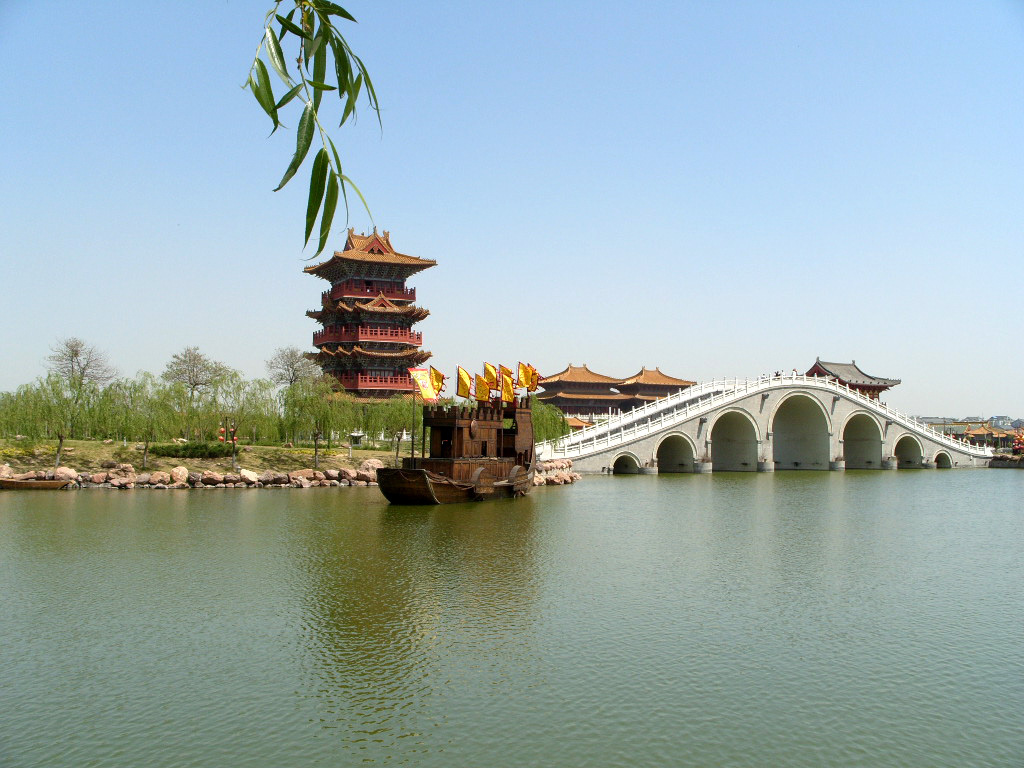
\includegraphics[scale=0.4]{figures/timg.jpg}
\end{figure}

\subsection{提高频谱利用效率的方法}
\begin{table}
    \centering
    \caption{这是第一个表格}
    \begin{tabular}{cccc}
        \toprule
        & \multicolumn{3}{c}{Numbers} \\
        \cmidrule{2-4}
        & 1 & 2 & 3 \\
        \midrule
        Alphabet & A & B & C \footnotemark \\
        Roman & I & II& III \\
    \bottomrule
    \end{tabular}
    
\end{table}
\footnotetext{表格里的字母是英文字母}
记忆伸向久远的过去,我再次触摸到你的呼吸。那是一个凄冷的早春,我身无分文,孑然立于城市街头。我在寒风中颤栗,也在寒风中绝望,我选择了一个失败者所能选择的结局:自杀 。当我横卧于铁轨上等待即将呼啸而至的列车时,你的强有力的大手一把把我拽离铁轨,并把我牵引入你的值班室。室内的炉火烘热了我的身体,你温润的话语烘热了我的心灵。我吃着你给我打来的饭菜,泪如雨下。你给了我五十块钱,劝我回家。最终你还是不放心,又一路陪同我到火车站,直到看着我进了站,你才放心离去
\section{认知无线电概述}
由于工作的关系,我和你被拉到同一个工作群里。我爱写作,每有新作出炉,总会发至群里供大家评点。你总是先给我回一串大大的赞,然后在软文后面写上你的阅读感受。一来二去,我们成了“朋友”。你说,你很敬佩我的高雅,想送给我一个礼物。我心生感动,但也只是当做逢场的恭维,不以为意。没想到,五天之后,我收到了来自你的快递。急急打开,原来是厚厚三大本书:日本儒学泰斗冈田武彦先生的心血力作《王阳明大传》全册。瞬间,我忍不住潸然泪下。不仅为你的倾心相赠,更为你的心细如发,我仅仅截图了我的电子书目发给你,里面有我喜欢的书《明朝一哥王阳明》,你竟然记住了。而今,我们依然是微信里的“朋友”,我只知道你是谁,你的名字叫赵冉,网名叫语冉心文。
\subsection{认知无线电的定义}
夜深沉,我却无心入睡。我于千里之外写下的关于你的文字,只为了让你知道,你如昙花一样惊艳的刹那芳华,已经深深绚烂了一颗孤独的心。你们不是这个社会的筋骨,但你们一定是这个社会的血肉
\subsection{认知无线电的关键技术}
风起叶落,年岁老去。这是在告诫人们,为什么不曾着此时拥有,好好把握属于自己的年华。秋风起时,不是单一用来相思和发愁的,而是用来思考和感悟的。



梧桐,银杏,合欢,秋天的风物在风中展示着自己的特性。城市与乡村,被任性的秋风抚摸。仿佛打翻了的调色盘,美丽的色彩把秋的意境拉长
\subsection{国内外认知无线电的研究现状}
乡间的落花生,砍高粱,掰玉米,割豆子,晒柿子。城市里,公园水边的芦苇在秋天诉说着,垂柳摆动着枝条,水草安静。出来散步的人群,吹着凉风,惬意而舒适,有人由衷说一句:“生活真的很美好!”



这么美好的生活,我们为什么要哀愁呢?应该尽情欢笑,尽管生活它有太多不如意,可是我们依旧满怀梦想。有梦就去追赶,趁着山高路长。尽管命运总是会捉弄人,可是我们依旧拥有爱与温暖。



路边的水吧,传来点唱机的音乐。秋风下,一点点灯火的昏黄,有着诗意的朦胧。此时此境,我路过它的美丽。不由得叹道:“人们总是渴望着诗和远方。却不能看见自己眼前的生活,就有着诗意的所在,和远方的期待。
\section{论文内容及结构}
\begin{figure}
    \centering
    \caption{这是第二张图片}
    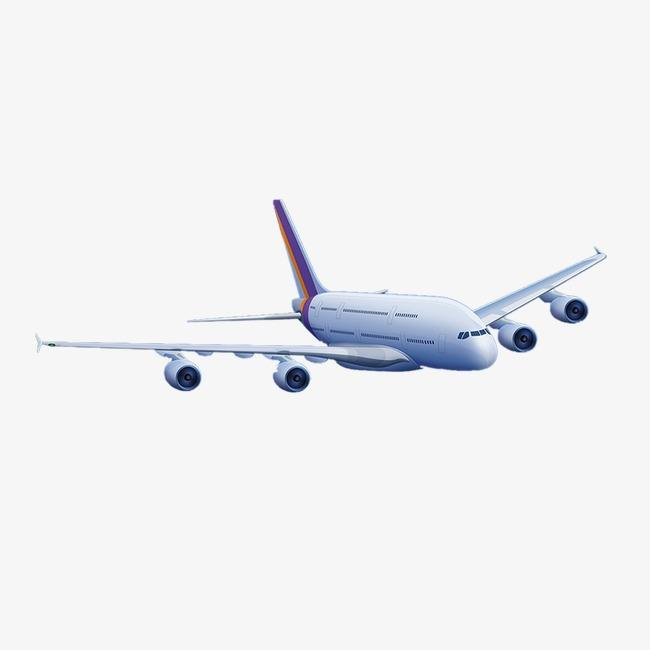
\includegraphics[scale=0.4]{figures/timg1.jpg}
\end{figure}
深有同感。多年前认识一个朋友,在外地工作。那时的联系方式主要是电话,原本节俭的他,却会在陌生的街头,日日给家中的妻儿挂一通电话。后来聚会时,他讲起自己的漂泊,说到此处,我们问为什么。



朋友很实在,他说:“这样我们一家人,会感觉每天生活在一起。”直至今天,我才读懂他对生活的理解。对生活深情的人,会在时间中种植深情。







秋风已起,思念与愁绪,深情与厚意,都在其中。我们都是风的孩子,乘着它的翅膀在人间飞翔。我时时告诫自己:“珍重待秋风!”
秋风已起,思念与愁绪,深情与厚意,都在其中。我们都是风的孩子,乘着它的翅膀在人间飞翔
秋风已起,思念与愁绪,深情与厚意,都在其中。我们都是风的孩子,乘着它的翅膀在人间飞翔秋风已起,思念与愁绪,深情与厚意,都在其中。我们都是风的孩子,乘着它的翅膀在人间飞翔
秋风已起,思念与愁绪,深情与厚意,都在其中。我们都是风的孩子,乘着它的翅膀在人间飞翔秋风已起,思念与愁绪,深情与厚意,都在其中。我们都是风的孩子,乘着它的翅膀在人间飞翔
秋风已起,思念与愁绪,深情与厚意,都在其中。我们都是风的孩子,乘着它的翅膀在人间飞翔秋风已起,思念与愁绪,深情与厚意,都在其中。我们都是风的孩子,乘着它的翅膀在人间飞翔
秋风已起,思念与愁绪,深情与厚意,都在其中。我们都是风的孩子,乘着它的翅膀在人间飞翔秋风已起,思念与愁绪,深情与厚意,都在其中。我们都是风的孩子,乘着它的翅膀在人间飞翔
秋风已起,思念与愁绪,深情与厚意,都在其中。我们都是风的孩子,乘着它的翅膀在人间飞翔
秋风已起,思念与愁绪,深情与厚意,都在其中。我们都是风的孩子,乘着它的翅膀在人间飞翔
秋风已起,思念与愁绪,深情与厚意,都在其中。我们都是风的孩子,乘着它的翅膀在人间飞翔
秋风已起,思念与愁绪,深情与厚意,都在其中。我们都是风的孩子,乘着它的翅膀在人间飞翔
秋风已起,思念与愁绪,深情与厚意,都在其中。我们都是风的孩子,乘着它的翅膀在人间飞翔
秋风已起,思念与愁绪,深情与厚意,都在其中。我们都是风的孩子,乘着它的翅膀在人间飞翔
秋风已起,思念与愁绪,深情与厚意,都在其中。我们都是风的孩子,乘着它的翅膀在人间飞翔秋风已起,思念与愁绪,深情与厚意,都在其中。我们都是风的孩子,乘着它的翅膀在人间飞翔
秋风已起,思念与愁绪,深情与厚意,都在其中。我们都是风的孩子,乘着它的翅膀在人间飞翔
秋风已起,思念与愁绪,深情与厚意,都在其中。我们都是风的孩子,乘着它的翅膀在人间飞翔
秋风已起,思念与愁绪,深情与厚意,都在其中。我们都是风的孩子,乘着它的翅膀在人间飞翔
秋风已起,思念与愁绪,深情与厚意,都在其中。我们都是风的孩子,乘着它的翅膀在人间飞翔
秋风已起,思念与愁绪,深情与厚意,都在其中。我们都是风的孩子,乘着它的翅膀在人间飞翔

秋风已起,思念与愁绪,深情与厚意,都在其中。我们都是风的孩子,乘着它的翅膀在人间飞翔
秋风已起,思念与愁绪,深情与厚意,都在其中。我们都是风的孩子,乘着它的翅膀在人间飞翔
秋风已起,思念与愁绪,深情与厚意,都在其中。我们都是风的孩子,乘着它的翅膀在人间飞翔
秋风已起,思念与愁绪,深情与厚意,都在其中。我们都是风的孩子,乘着它的翅膀在人间飞翔
秋风已起,思念与愁绪,深情与厚意,都在其中。我们都是风的孩子,乘着它的翅膀在人间飞翔
秋风已起,思念与愁绪,深情与厚意,都在其中。我们都是风的孩子,乘着它的翅膀在人间飞翔

秋风已起,思念与愁绪,深情与厚意,都在其中。我们都是风的孩子,乘着它的翅膀在人间飞翔
秋风已起,思念与愁绪,深情与厚意,都在其中。我们都是风的孩子,乘着它的翅膀在人间飞翔
秋风已起,思念与愁绪,深情与厚意,都在其中。我们都是风的孩子,乘着它的翅膀在人间飞翔
秋风已起,思念与愁绪,深情与厚意,都在其中。我们都是风的孩子,乘着它的翅膀在人间飞翔
秋风已起,思念与愁绪,深情与厚意,都在其中。我们都是风的孩子,乘着它的翅膀在人间飞翔
秋风已起,思念与愁绪,深情与厚意,都在其中。我们都是风的孩子,乘着它的翅膀在人间飞翔

秋风已起,思念与愁绪,深情与厚意,都在其中。我们都是风的孩子,乘着它的翅膀在人间飞翔
秋风已起,思念与愁绪,深情与厚意,都在其中。我们都是风的孩子,乘着它的翅膀在人间飞翔
